\section{Çalışma Örnekleri}
Yazılımı kullanmak için ilk olarak 'yıl' bilgisi seçilir. Daha sonra o yıla ait modeli çalıştırabilmek için girilmesi gereken özellikler kullanıcıdan istenecektir. Bilgiler girildikten sonra en altta bulunan 'Tahmin Et' butonu ile tahmin işlemi gerçekleştirilir.

\begin{figure}[h]
  \centering
  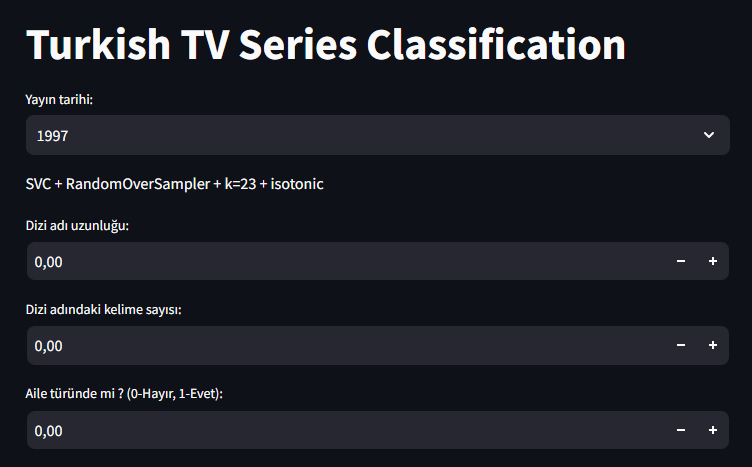
\includegraphics[width=1.0\textwidth]{ekran.png}
  \caption{Tahmin ekranı.}
  \label{fig:resim_2}
\end{figure}

\newpage